
In this document we have described a search for the Standard Model Higgs boson
decaying to a pair of $Z$ bosons.  We analysed the final state with two leptons consistent with
the Z decay ($ee$ or $\mu\mu$) and large MET from the decay of the second $Z$ to neutrinos.
This analysis is sensitive to the Standard Model Higgs boson at large Higgs boson mass.
We have also performed an analysis of the dilepton+MET final state where
the Higgs boson decays to a pair of $W$ bosons \cite{HWW2011ANFULL}.
While both analyses share the same dilepton+MET final state, the former 
requires a same flavor dilepton pair consistent with the $Z$ mass,
the latter excludes these events. 
The combination of the two analyses can increase the sensitivity                   
of the dilepton+MET final state to the Standard Model Higgs boson
over a larger mass range by using all selected dilepton+MET events.

The expected and observed limits for the $ZZ$ analysis described in this document
are given in Table \ref{tab:hzz_acls_bayes}.  The expected and observed limits for the
$WW$ analysis are given in Table \ref{tab:hww_acls_bayes}.  In both cases we 
tabulate the results calculated with the Asymptotic CLs and Bayesian methods.
The limit from both analyses combined is given in Table \ref{fig:combinarion_bayes_fig}
and Figures \ref{fig:combinarion_bayes_fig} and \ref{fig:combinarion_asym_fig}.

In $ZZ$ analysis we exclude
the presence of the Standard Model Higgs boson at 95\% C.L. in the mass range
[275-455] GeV/c$^{2}$ using the $M_T$ shape analysis.
In the $WW$ analysis we exclude the Standard Model Higgs in the mass range [128-375]~GeV/c$^{2}$.
We find that by combining the two analyses in the $2\ell2\nu$ final state we
can exclude the Standard Model Higgs in the mass range [128, 500]~GeV/c$^{2}$.

\vspace{20pt}

%
%
%

%%%%%%%%%%%%%%%%%%%%%%%%%%%%%%
% HZZ ONLY
%%%%%%%%%%%%%%%%%%%%%%%%%%%%%%% 
\begin{table}[!htbp]
\begin{center}
\begin{tabular}{ccccc}
\hline\hline
Mass & Observed & Median Expected & [-$\sigma$, +$\sigma$] & [-2$\sigma$, +2$\sigma$]\\\hline
\hline
\multicolumn{5}{c} {Asymptotic CLs} \\
\hline
250 & 1.50 & 1.38 & [1.00, 1.92] & [0.75, 2.56] \\
300 & 0.66 & 0.93 & [0.67, 1.29] & [0.51, 1.72] \\ 
350 & 0.55 & 0.63 & [0.45, 0.87] & [0.34, 1.16] \\
400 & 0.54 & 0.63 & [0.46, 0.88] & [0.34, 1.17] \\
500 & 1.58 & 1.08 & [0.78, 1.50] & [0.58, 1.99] \\
600 & 2.41 & 2.23 & [1.61, 3.10] & [1.21, 4.12] \\
\hline
\multicolumn{5}{c} {Bayesian} \\
\hline
250 & 1.51 & 1.45 & [1.04, 2.17] & [0.76, 3.03] \\
300 & 0.70 & 1.05 & [0.72, 1.55] & [0.50, 2.32] \\
350 & 0.58 & 0.71 & [0.49, 1.03] & [0.35, 1.48] \\
400 & 0.71 & 0.70 & [0.49, 1.03] & [0.36, 1.58] \\
500 & 1.70 & 1.24 & [0.87, 1.81] & [0.65, 2.53] \\
600 & 2.83 & 2.67 & [1.91, 3.93] & [1.40, 5.92] \\
\hline\hline
\end{tabular}
\end{center}
\caption{The observed and expected cross section ratio limits as a function 
of the Higgs mass, together with the 1/2-$\sigma$ uncertainty bands obtained in the 
$M_T$ shape analysis for the $ZZ\rightarrow\ell\ell\nu\nu$ decay channel.}
\label{tab:hzz_acls_bayes}
\end{table}
%%%%%%%%%%%%%%%%%%%%%%%%%%%%%%% 

%%%%%%%%%%%%%%%%%%%%%%%%%%%%%%
% HWW ONLY
%%%%%%%%%%%%%%%%%%%%%%%%%%%%%%% 
\begin{table}[!htbp]
\begin{center}
\begin{tabular}{ccccc}
\hline\hline
Mass & Observed & Median Expected & [-$\sigma$, +$\sigma$] & [-2$\sigma$, +2$\sigma$]\\\hline
\hline
\multicolumn{5}{c} {Asymptotic CLs} \\
\hline
115 & 4.61 & 2.58 & [1.86, 3.59] & [1.38, 4.81] \\
120 & 2.44 & 1.51 & [1.09, 2.11] & [0.81, 2.82] \\
130 & 0.80 & 0.73 & [0.53, 1.01] & [0.39, 1.36] \\
140 & 0.61 & 0.43 & [0.31, 0.60] & [0.23, 0.80] \\
150 & 0.42 & 0.30 & [0.22, 0.42] & [0.16, 0.56] \\
160 & 0.24 & 0.19 & [0.13, 0.26] & [0.10, 0.35] \\
170 & 0.26 & 0.20 & [0.14, 0.27] & [0.11, 0.37] \\
180 & 0.32 & 0.26 & [0.19, 0.36] & [0.14, 0.48] \\
190 & 0.32 & 0.38 & [0.27, 0.53] & [0.20, 0.71] \\
200 & 0.46 & 0.50 & [0.36, 0.69] & [0.27, 0.93] \\
250 & 0.71 & 0.94 & [0.68, 1.31] & [0.51, 1.76] \\
300 & 0.83 & 1.03 & [0.74, 1.44] & [0.55, 1.93] \\
350 & 0.93 & 0.93 & [0.67, 1.30] & [0.50, 1.74] \\
400 & 1.36 & 0.98 & [0.71, 1.36] & [0.53, 1.83] \\
500 & 1.26 & 1.85 & [1.34, 2.58] & [0.99, 3.46] \\
600 & 2.33 & 3.76 & [2.71, 5.23] & [2.02, 7.01] \\
\hline
\multicolumn{5}{c} {Bayesian} \\
\hline
115 & 4.64 & 2.46 & [1.59, 3.79] & [1.09, 5.50] \\
120 & 2.28 & 1.38 & [0.88, 2.19] & [0.56, 3.17] \\
130 & 0.84 & 0.67 & [0.40, 1.02] & [0.24, 1.55] \\
140 & 0.64 & 0.39 & [0.23, 0.60] & [0.14, 0.94] \\
150 & 0.44 & 0.27 & [0.16, 0.41] & [0.10, 0.60] \\
160 & 0.22 & 0.14 & [0.09, 0.21] & [0.06, 0.32] \\
170 & 0.24 & 0.15 & [0.09, 0.24] & [0.06, 0.35] \\
180 & 0.24 & 0.22 & [0.13, 0.34] & [0.08, 0.51] \\
190 & 0.38 & 0.33 & [0.20, 0.54] & [0.13, 0.85] \\
200 & 0.51 & 0.46 & [0.28, 0.72] & [0.18, 1.10] \\
250 & 0.79 & 0.87 & [0.52, 1.38] & [0.33, 2.05] \\
300 & 1.00 & 0.95 & [0.57, 1.54] & [0.37, 2.30] \\
350 & 1.02 & 0.84 & [0.53, 1.40] & [0.34, 2.07] \\
400 & 1.09 & 0.93 & [0.59, 1.50] & [0.37, 2.18] \\
500 & 1.20 & 1.76 & [1.17, 2.68] & [0.71, 3.91] \\
600 & 3.27 & 3.36 & [2.18, 5.67] & [1.39, 8.73] \\
\hline\hline
\end{tabular}
\end{center}
\caption{The observed and expected cross section ratio limits as a function
of the Higgs mass, together with the 1/2-$\sigma$ uncertainty bands obtained in the 
$M_T$ shape analysis for the $WW\rightarrow\ell\nu\ell\nu$ decay channel.}
\label{tab:hww_acls_bayes}
\end{table}
%%%%%%%%%%%%%%%%%%%%%%%%%%%%%%% 

%%%%%%%%%%%%%%%%%%%%%%%%%%%%%%
% HWW + HZZ
%%%%%%%%%%%%%%%%%%%%%%%%%%%%%%% 
\begin{table}[!htbp]
\begin{center}
\begin{tabular}{ccccc}
\hline\hline
Mass & Observed & Median Expected & [-$\sigma$, +$\sigma$] & [-2$\sigma$, +2$\sigma$]\\\hline
\hline 
\multicolumn{5}{c} {Asymptotic CLs} \\
\hline
115 & 4.61 & 2.58 & [1.86, 3.59] & [1.38, 4.81] \\
120 & 2.44 & 1.51 & [1.09, 2.11] & [0.81, 2.82] \\
130 & 0.80 & 0.73 & [0.53, 1.01] & [0.39, 1.36] \\
140 & 0.61 & 0.43 & [0.31, 0.60] & [0.23, 0.80] \\
150 & 0.42 & 0.30 & [0.22, 0.42] & [0.16, 0.56] \\
160 & 0.24 & 0.19 & [0.13, 0.26] & [0.10, 0.35] \\
170 & 0.26 & 0.20 & [0.14, 0.27] & [0.11, 0.37] \\
180 & 0.28 & 0.26 & [0.19, 0.36] & [0.14, 0.48] \\
190 & 0.38 & 0.38 & [0.27, 0.53] & [0.20, 0.71] \\
200 & 0.49 & 0.50 & [0.36, 0.69] & [0.27, 0.93] \\
250 & 0.64 & 0.81 & [0.58, 1.13] & [0.43, 1.51] \\
300 & 0.58 & 0.70 & [0.50, 0.97] & [0.37, 1.30] \\
350 & 0.47 & 0.53 & [0.38, 0.73] & [0.28, 0.98] \\
400 & 0.61 & 0.54 & [0.39, 0.75] & [0.29, 1.00] \\
500 & 0.90 & 0.92 & [0.66, 1.28] & [0.49, 1.71] \\
600 & 1.38 & 1.86 & [1.34, 2.58] & [1.00, 3.46] \\
\hline
\multicolumn{5}{c} {Bayesian} \\
\hline
115 & 4.64 & 2.49 & [1.60, 3.81] & [1.08, 5.51] \\
120 & 2.28 & 1.39 & [0.90, 2.26] & [0.62, 3.30] \\
130 & 0.84 & 0.69 & [0.41, 1.09] & [0.26, 1.53] \\
140 & 0.64 & 0.38 & [0.24, 0.63] & [0.15, 0.88] \\
150 & 0.44 & 0.27 & [0.16, 0.42] & [0.10, 0.62] \\
160 & 0.22 & 0.13 & [0.09, 0.21] & [0.06, 0.32] \\
170 & 0.24 & 0.16 & [0.09, 0.24] & [0.06, 0.36] \\
180 & 0.24 & 0.22 & [0.13, 0.34] & [0.08, 0.52] \\
190 & 0.38 & 0.34 & [0.21, 0.56] & [0.13, 0.83] \\
200 & 0.51 & 0.45 & [0.27, 0.71] & [0.18, 1.00] \\
250 & 0.80 & 0.77 & [0.42, 1.26] & [0.28, 1.97] \\
300 & 0.70 & 0.68 & [0.43, 1.07] & [0.26, 1.69] \\
350 & 0.38 & 0.51 & [0.32, 0.82] & [0.21, 1.29] \\
400 & 0.79 & 0.53 & [0.34, 0.79] & [0.25, 1.38] \\
500 & 0.92 & 0.90 & [0.58, 1.37] & [0.39, 1.99] \\
600 & 1.62 & 1.86 & [1.18, 3.04] & [0.72, 4.81] \\
\hline\hline 
\end{tabular}
\end{center}
\caption{The observed and expected cross section ratio limits as a function
of the Higgs mass, together with the 1/2-$\sigma$ uncertainty bands obtained in the
combination of the $WW\rightarrow\ell\nu\ell\nu$ and $ZZ\rightarrow\ell\ell\nu\nu$ 
decay channels.}
\label{tab:hzz_hww_combination}
\end{table}

%%%%%%%%%%%%%%%%%%%%%%%%%%%%%
\begin{figure}[!htbp]
\subfigure[HWW]{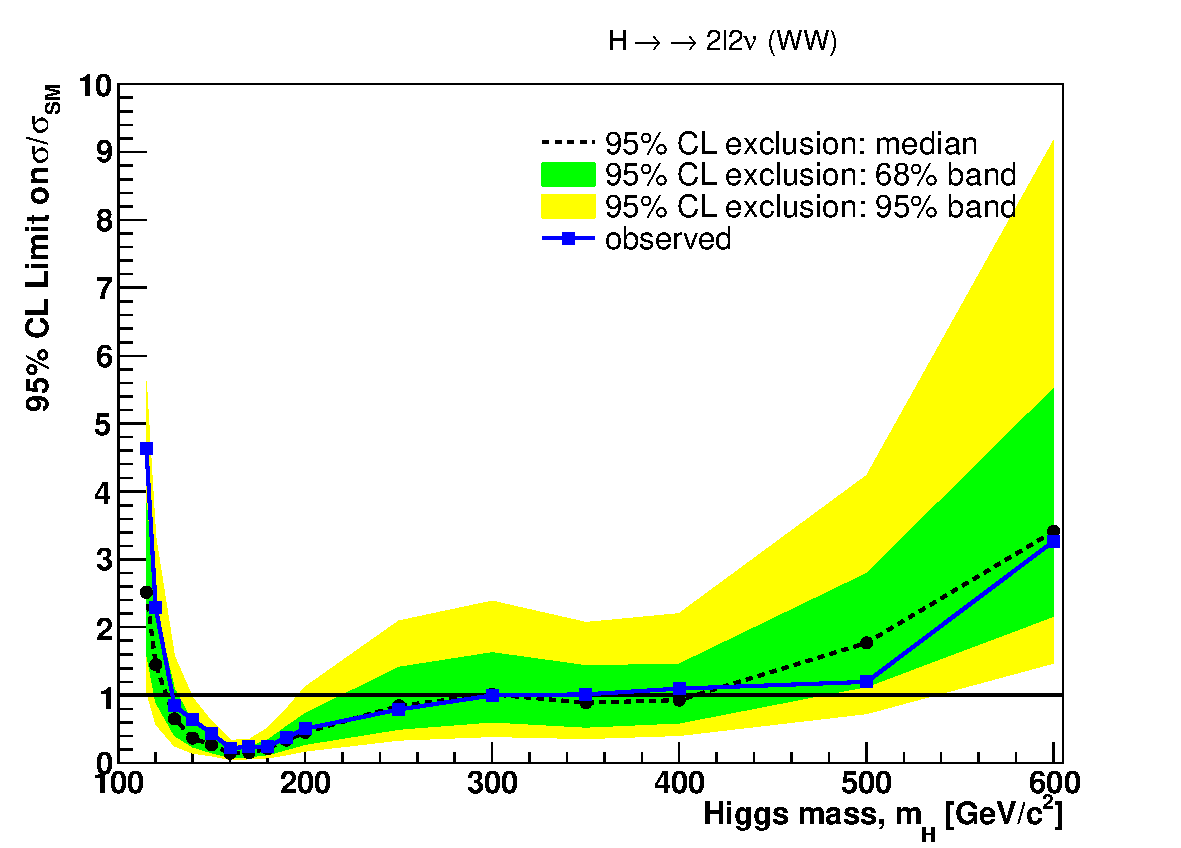
\includegraphics[width=0.55\textwidth]{figures/supercard_hww-Bayesian.pdf}}
\subfigure[HWW+HZZ]{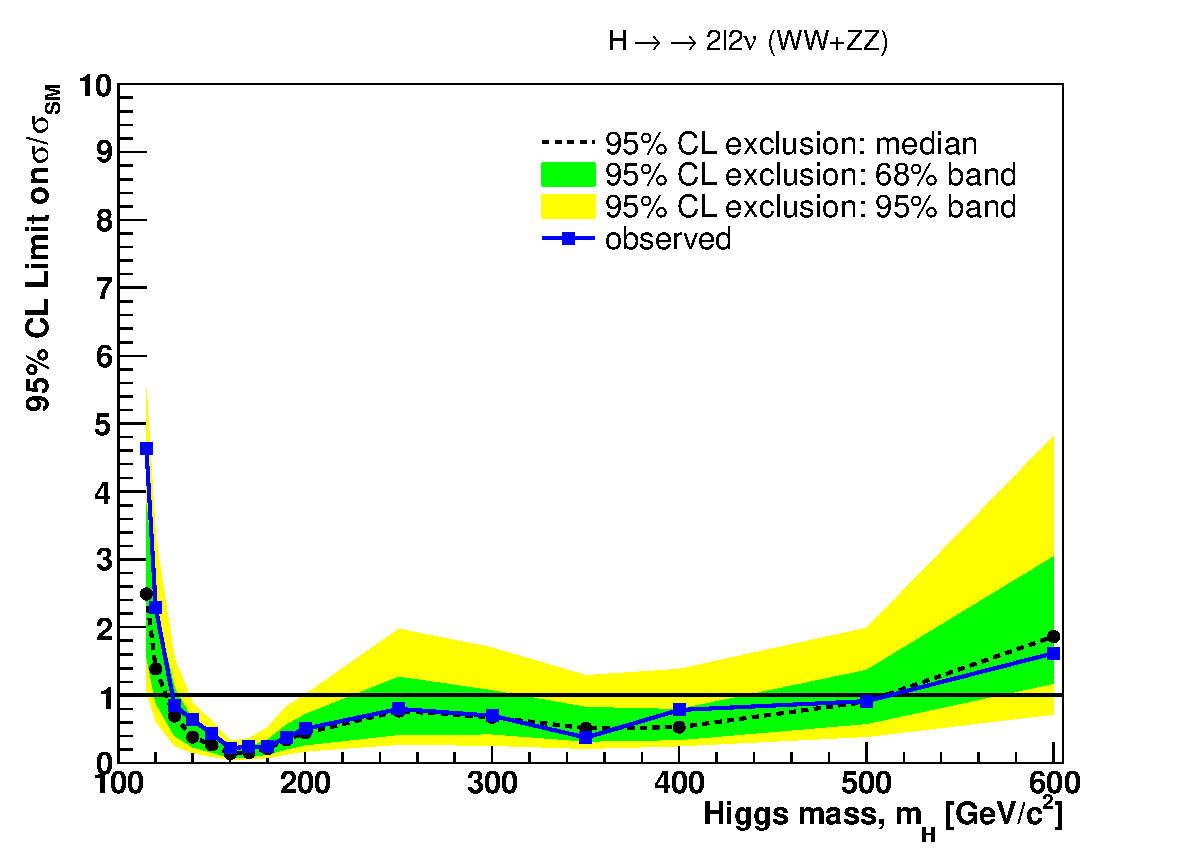
\includegraphics[width=0.55\textwidth]{figures/supercard_h-Bayesian.pdf}}
\caption{The expected and observed 95\% C.L. upper limits on the
Standard Model production cross section in the $WW\rightarrow\ell\nu\ell\nu$ channel (left)
and in combination with the $ZZ\rightarrow\ell\ell\nu\nu$ channel (right).
The limtis shown are calculated using the Bayesian method.}
\label{fig:combinarion_bayes_fig}
%\end{figure}
%%%%%%%%%%%%%%%%%%%%%%%%%%%%%
%
%%%%%%%%%%%%%%%%%%%%%%%%%%%%%
%\begin{figure}[!htbp]
\subfigure[HWW]{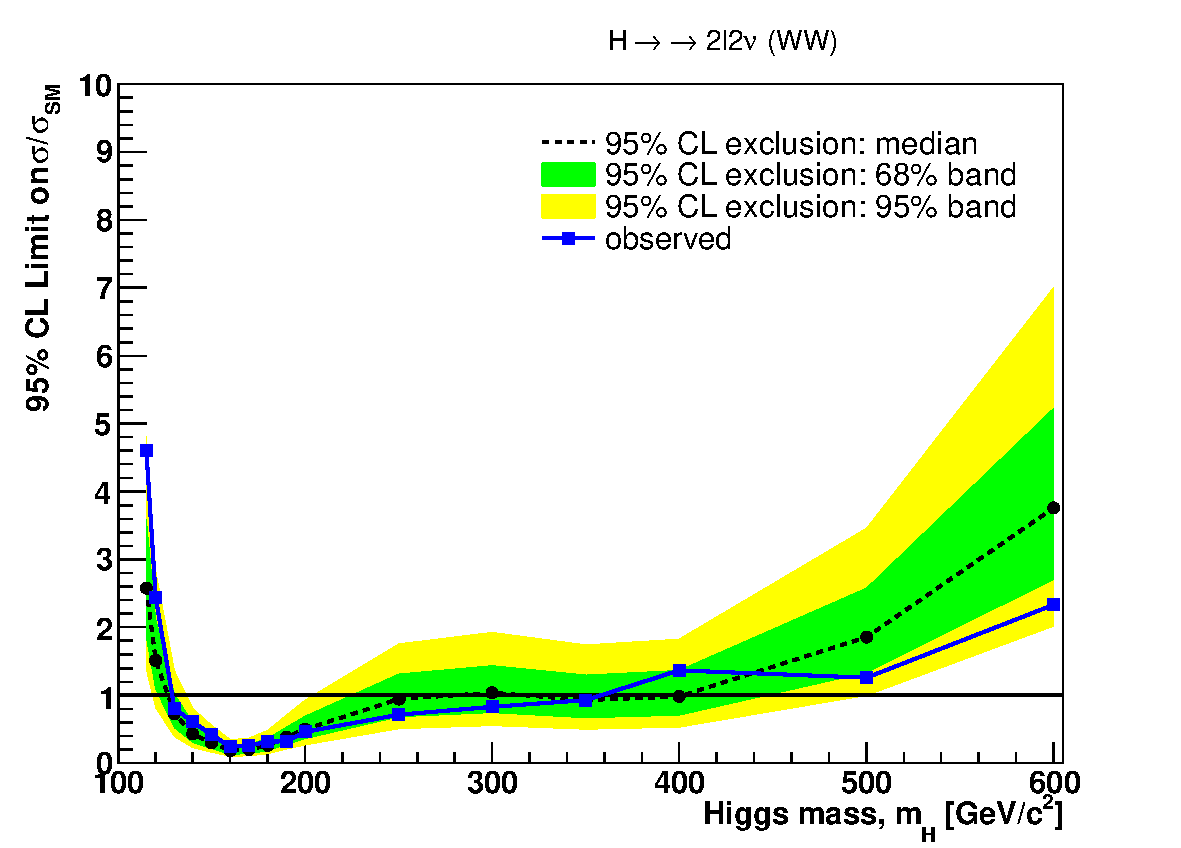
\includegraphics[width=0.55\textwidth]{figures/supercard_hww-CLs-asymptotic.pdf}}
\subfigure[HWW+HZZ]{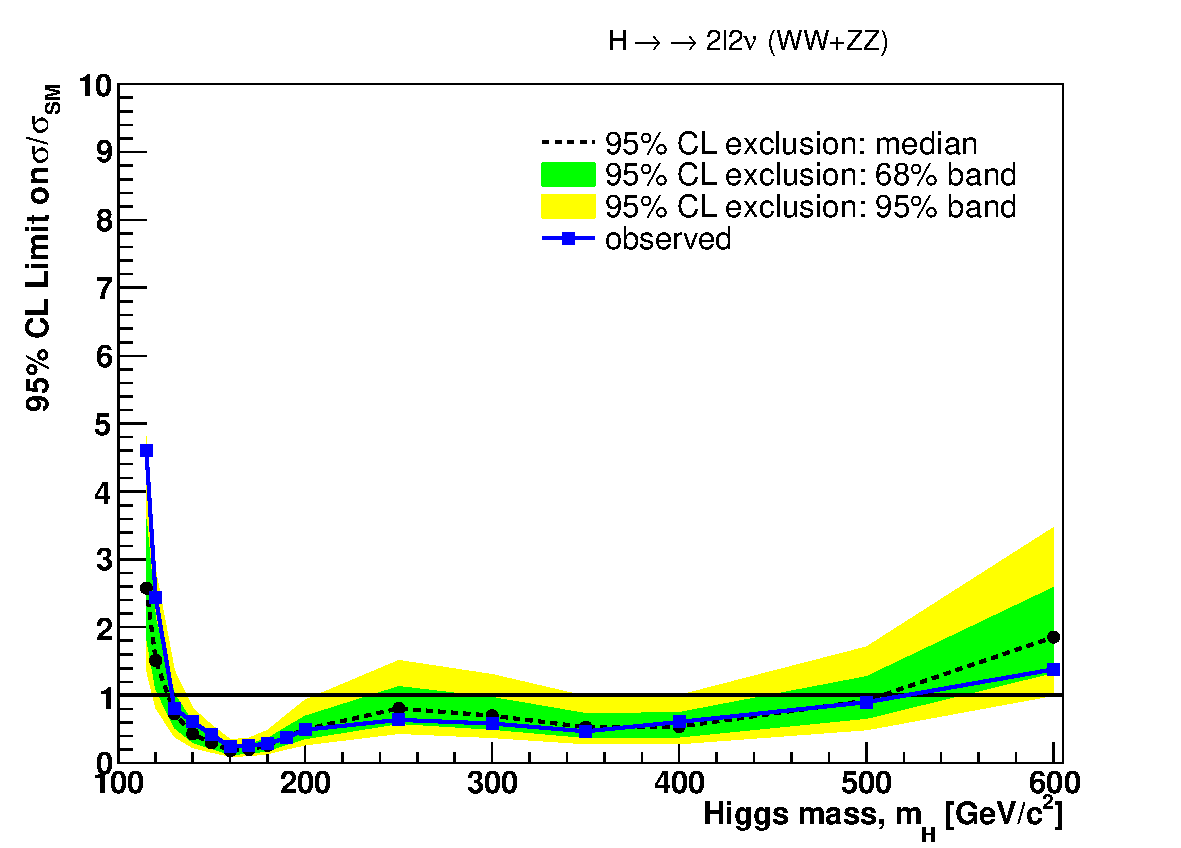
\includegraphics[width=0.55\textwidth]{figures/supercard_h-CLs-asymptotic.pdf}}
\caption{The expected and observed 95\% C.L. upper limits on the 
Standard Model production cross section in the $WW\rightarrow\ell\nu\ell\nu$ channel (left)
and in combination with the $ZZ\rightarrow\ell\ell\nu\nu$ channel (right).
The limits shown are calculated using the asymptotic CLs method.}
\label{fig:combinarion_asym_fig}
\end{figure}
%%%%%%%%%%%%%%%%%%%%%%%%%%%%%

